\documentclass[a4paper,12pt]{article} 
\usepackage[utf8]{inputenc}
\usepackage{graphicx}
\usepackage{wrapfig}
\usepackage{tabularx}
\usepackage{lipsum}
\usepackage{url}
\usepackage{hyperref}
\usepackage{pgfgantt}
\usepackage{enumitem}
\usepackage{indentfirst}
\linespread{1.5}
\usepackage{geometry}
\usepackage{float} 
\usepackage{times}
\geometry{left= 1.5 in,
            right= 1 in,
            top= 1 in,
            bottom= 1 in}
\usepackage{amsmath}
\usepackage{anyfontsize}
\usepackage[hidelinks]{hyperref}
\usepackage{hyperref}
\usepackage[
    backend=biber,
    style=ieee,
    sorting=none
]{biblatex}

\addbibresource{bibliography.bib}
\pagenumbering{gobble} 
\setlength{\parindent}{0pt}


\begin{document}

\begin{titlepage}
	\begin{center}
	
	\large %14pt
	A Minor Project Mid-term Report on
	
	\huge %24pt
	\textbf{Automated Two-Wheeler Violation Detection and E-Challan System using YoloV8 with OpenCV}

	\vfill
	
	\large %14pt
	Submitted in Partial Fulfillment of the \\ 
	Requirements for the Degree of \\ 
	\textbf {Bachelor of Engineering in Computer Engineering} \\
	under Pokhara University
	
	\vfill
	
	Submitted by: \\ 
        \textbf {Abishek Khadka, 231303} \\
        \textbf {Ishbarna Kafle, 231317} \\
	\textbf {Madan Belbase, 231323} \\

	\vfill
	
        Under the supervision of: \\
	\textbf{Er. Rishi K. Marseni}
	
	\vfill
	    \vspace{12mm}
        
	Date: \\
	\textbf {24 January 2026}
	
	\vfill
	
	\end{center}
	
	\begin{wrapfigure}{L}{0.2\textwidth}
	\centering
	
\includegraphics[width=0.2\textwidth]{figures/system/college-logo.png}
	\end{wrapfigure}
	
	\fontfamily{phv}\selectfont
	
	\textbf {Department of Computer Engineering}  
	
	% \Large %17pt
        \LARGE %21pt
	\textbf {NEPAL COLLEGE OF} 
	
	\LARGE %21pt
	\textbf {\underline {INFORMATION TECHNOLOGY} }
	
	\small %11 pt
	Balkumari, Lalitpur, Nepal
	
	
\end{titlepage}

% \newpage
% \pagenumbering{Roman}
% \addcontentsline{toc}{section}
% {\numberline{}Acknowledgementt}
% \section*{Acknowledgement}
% %\input{chapters/acknowledgement}\\\\
% \newpage
% Will use this section for final

\newpage
\pagenumbering{Roman}
\addcontentsline{toc}{section}{Abstract}
\section*{Abstract}
This mid-term report presents the design and implementation progress of an Automated Two-Wheeler Violation Detection and E-Challan System using YOLOv8 and OpenCV. The project aims to detect common traffic violations related to two-wheelers, such as helmet non-compliance and improper number plate visibility, from video streams captured by roadside cameras. The proposed system performs real-time object detection for riders and helmets, tracks detected vehicles across frames, localizes the license plate region, and extracts the registration number using optical character recognition. Based on predefined violation rules, the system generates a digital e-challan containing evidence frames, timestamp, detected violation type, and extracted plate number. This report discusses the problem context, objectives, methodology, system architecture, and tasks completed so far, along with the remaining work plan and evaluation strategy. Preliminary experiments show that YOLOv8-based detection provides promising accuracy and speed for real-time deployment on mid-range hardware.


\newpage
\tableofcontents

\newpage
\listoffigures

\newpage
\listoftables

\newpage
\pagenumbering{arabic}

\section{Introduction}
Traffic rule violations by two-wheelers—especially helmet non-compliance—remain a major contributor to road injuries and fatalities. Manual monitoring and challan issuance are time-consuming, costly, and often inconsistent, particularly in areas with high traffic density. With the increasing availability of surveillance cameras and advances in computer vision, automated enforcement systems can assist traffic authorities by continuously monitoring roads, identifying violations, and generating evidence-backed challans.

This project focuses on developing an automated two-wheeler violation detection pipeline using YOLOv8 for object detection and OpenCV for video processing. The system targets violations such as riding without a helmet, multiple riders (triple riding) where applicable, and number plate-related issues (e.g., missing or unclear plates). Once a violation is detected, the system extracts the license plate number using OCR and generates an e-challan record with supporting metadata. The overall goal is to build a practical prototype that can operate on recorded videos or live camera feeds and produce results suitable for further integration with an authority-side database or dashboard.


\subsection{Problem Statement}
Two-wheeler traffic violations such as riding without a helmet and improper/missing number plates are frequently observed in urban roads. Existing enforcement practices rely heavily on manual checking or sporadic checkpoints, which cannot provide continuous coverage. Manual approaches also face limitations including human error, delayed challan issuance, and difficulties in maintaining consistent evidence.

Therefore, the problem addressed in this project is to design and implement an automated system that (i) detects two-wheelers and relevant safety attributes (helmet usage), (ii) identifies whether a traffic violation has occurred based on defined rules, (iii) extracts the vehicle registration number from the number plate, and (iv) generates an e-challan entry with adequate evidence and timestamps.


\newpage

\subsection{Project Objectives}
The primary objective of this project is to design and develop a Smart Rider Monitoring \& Violation Detection System using computer vision and deep learning techniques for automated traffic surveillance.

The specific objectives of the project are as follows:
\begin{enumerate}
\item To detect motorcycles and riders from live video streams and identify specific traffic violations, namely helmet non-compliance and triple-riding.
\item To recognize vehicle number plates using Optical Character Recognition (OCR) for accurate violator identification.
\item To provide a real-time monitoring dashboard that automatically generates violation records and e-challans with supporting digital evidence to improve law enforcement efficiency.
\end{enumerate}

\newpage

\subsection{Significance of the study}
An automated violation detection and e-challan system can support traffic authorities by reducing the dependency on manual monitoring and improving consistency in enforcement. Continuous camera-based monitoring can increase the probability of detecting violations while also creating a transparent evidence trail for challan issuance.

From a technical perspective, this project demonstrates the practical application of deep learning-based object detection (YOLOv8) combined with OpenCV-based video processing and OCR for a real-world public safety use case. The developed prototype and evaluation can serve as a baseline for future work involving multi-camera deployments, database-backed dashboards, and integration with smart city infrastructure.


\newpage

\subsection{Scope and Limitation}
\textbf{Scope:}
\begin{itemize}[leftmargin=*]
  \item Detection of two-wheelers, riders, and helmets from recorded video and/or live camera feed.
  \item Rule-based identification of selected violations (primary focus: helmet non-compliance).
  \item Number plate localization and OCR-based plate number extraction.
  \item Generation of a prototype e-challan output (e.g., JSON/CSV record with evidence frames).
\end{itemize}

\textbf{Limitations:}
\begin{itemize}[leftmargin=*]
  \item Performance may degrade under poor lighting, occlusion, motion blur, and low-resolution footage.
  \item OCR accuracy depends on plate visibility, camera angle, and plate quality.
  \item The prototype does not cover all possible traffic violations and legal edge cases.
  \item Integration with official government databases, authentication, and payment gateways is outside the scope of the mid-term prototype.
\end{itemize}

\newpage

\section{Literature Review}
Road traffic violations are a major cause of accidents and fatalities worldwide. With the advancement of computer vision and deep learning technologies, automated traffic monitoring systems have gained significant attention for detecting violations such as helmetless riding, triple riding, mobile phone usage while driving, and vehicle identification through Automatic Number Plate Recognition (ANPR).

Recent studies have demonstrated the effectiveness of deep learning-based object detection models for traffic surveillance applications. Among various approaches, the YOLO (You Only Look Once) family of models has emerged as one of the most widely adopted techniques due to its high detection accuracy and real-time processing capability. Chen et al. proposed a deep learning framework for detecting helmet-rule violations among motorcyclists and reported promising results under complex traffic conditions \cite{Chen2024}. Similarly, Said et al. enhanced helmet detection performance using an improved PerspectiveNet architecture integrated with EfficientNetV2, achieving high accuracy in motorcycle rider classification tasks \cite{Said2024}.

Helmet violation detection has been extensively studied because the use of helmets significantly reduces the risk of fatal injuries in motorcycle accidents. Most existing approaches follow a two-stage pipeline in which motorcycles and riders are first detected, followed by classification of helmet usage. Recent advancements in object detection and image classification have enabled reliable helmet detection even in crowded traffic scenes \cite{Chen2024, Said2024}.

Another important traffic violation is triple riding, which poses a serious safety risk for motorcycle users. Deshpande et al. developed a deep-learning-based framework capable of identifying motorcycles, counting riders, and detecting triple-riding violations from surveillance footage \cite{Deshpande2025}. Their work demonstrated that rider-count estimation can be effectively integrated with object detection systems, although challenges such as occlusion, varying camera angles, and image quality continue to affect performance.

The detection of mobile phone usage while riding or driving has also become an active area of research. Distracted driving caused by mobile phone usage contributes significantly to road accidents. Charef et al. proposed a computer vision approach based on YOLOv8 for detecting mobile phone usage among motorcycle riders \cite{Charef2025}. Their findings highlighted the difficulty of accurately identifying handheld devices due to object size, rider movement, and partial occlusions. Nevertheless, recent advances in deep learning have shown promising results for real-time distraction detection systems.

Automatic Number Plate Recognition (ANPR) is a critical component of intelligent traffic management systems. ANPR systems automatically detect vehicle registration plates and extract textual information using image processing, optical character recognition (OCR), and deep learning techniques. Modern ANPR solutions commonly employ object detection models such as YOLO for plate localization and convolutional neural networks for character recognition, achieving high accuracy under varying environmental conditions \cite{Du2013}.

Several countries have integrated ANPR systems with electronic traffic enforcement mechanisms to automate violation management. E-Challan systems digitally generate traffic tickets based on detected violations and maintain centralized violation records. Such systems reduce manual intervention, improve transparency, and increase enforcement efficiency. Automated enforcement frameworks combining violation detection, ANPR, and digital ticket generation have been successfully deployed in various smart traffic management applications \cite{Sharma2023}.

Despite significant progress in individual components such as helmet detection, triple-riding detection, mobile phone detection, and ANPR, most existing studies focus on a single violation type. Comprehensive systems capable of detecting multiple violations and automatically generating digital challans remain relatively limited. Furthermore, the performance of these systems often depends on the availability of high-quality datasets that accurately represent real-world traffic conditions. Therefore, the development of an integrated multi-violation detection and automated e-challan system remains an important research area in intelligent transportation systems.
\newpage

\section{Methodology}
The project follows an incremental prototyping approach. First, a baseline detection pipeline is built to identify two-wheelers and helmet usage in images. Next, the pipeline is extended to process video frames in real time, apply tracking to maintain object identity across frames, and apply violation rules. Finally, number plate extraction and e-challan generation are integrated to produce an end-to-end workflow.

The overall workflow is summarized as follows:
\begin{enumerate}[leftmargin=*]
  \item Capture video stream (recorded file or live feed) and extract frames.
  \item Run YOLOv8-based detection to identify relevant objects (two-wheeler, person, helmet, number plate region if modeled).
  \item Associate detections across frames using a tracking method (e.g., IOU-based tracking or a tracker such as SORT/DeepSORT).
  \item Determine violations using rule-based logic (e.g., rider detected without helmet for a stable sequence of frames).
  \item Crop the number plate region and apply OCR to extract text.
  \item Generate e-challan output with plate number, violation type, timestamp, and evidence images.
\end{enumerate}

\subsection{Software Development Lifecycle}
This project follows a simplified iterative SDLC:
\begin{itemize}[leftmargin=*]
  \item \textbf{Requirement Analysis:} Identify target violations (helmet), input sources (video), and expected outputs (e-challan record).
  \item \textbf{Design:} Define system modules---video ingestion, detection, tracking, violation logic, OCR, and report generation.
  \item \textbf{Implementation:} Develop modules using Python, Ultralytics YOLOv8, and OpenCV; integrate OCR.
  \item \textbf{Testing:} Validate on sample videos with different traffic density and lighting conditions; verify OCR outputs.
  \item \textbf{Evaluation:} Measure detection metrics and runtime performance (FPS), and document failure cases.
  \item \textbf{Iteration:} Tune models/thresholds, improve preprocessing, and refine rules based on observed errors.
\end{itemize}

\subsection{Technical Description}
\textbf{Tools and Libraries:}
\begin{itemize}[leftmargin=*]
  \item \textbf{YOLOv8 (Ultralytics):} Used for object detection due to its balance of speed and accuracy \cite{ultralyticsyolov8}.
  \item \textbf{OpenCV:} Used for video capture, frame processing, drawing annotations, cropping ROIs, and saving evidence frames \cite{opencv_library}.
  \item \textbf{OCR Engine:} Tesseract OCR (or an equivalent OCR model) is used to extract the registration number from the cropped number plate \cite{tesseract}.
\end{itemize}

\textbf{System Modules:}
\begin{enumerate}[leftmargin=*]
  \item \textbf{Frame Acquisition Module:} Reads frames from a video file or camera stream and applies resizing for consistent inference.
  \item \textbf{Detection Module:} Runs YOLOv8 on each frame to detect motorcycles/riders, helmets, and optionally number plate regions \cite{redmon2016yolo,ultralyticsyolov8}.
  \item \textbf{Tracking Module:} Maintains a track ID per vehicle/rider across consecutive frames to reduce duplicate challans.
  \item \textbf{Violation Decision Module:} Uses spatial relationships and temporal smoothing to reduce false positives.
  \item \textbf{OCR Module:} Applies preprocessing (grayscale, denoise, thresholding) before OCR to improve text extraction.
  \item \textbf{E-Challan Generation Module:} Stores a structured record containing plate number, violation type, time, and evidence.
\end{enumerate}

\subsection{E-Challan Generation}
When the system confirms a violation for a tracked two-wheeler, it generates an e-challan entry. Each challan record is designed to include:
\begin{itemize}[leftmargin=*]
  \item unique challan ID (auto-generated),
  \item date and time (timestamp from the video frame),
  \item detected violation type (e.g., helmet not detected),
  \item extracted vehicle number plate text,
  \item evidence image(s): original frame and/or cropped regions (rider/helmet/plate),
  \item confidence scores (detection confidence and OCR confidence when available).
\end{itemize}

For the prototype, challans are stored in a local structured format (CSV/JSON) along with a folder of evidence images. The e-challan output format is kept simple to allow future integration with a web dashboard or database.

\newpage
\newpage


\section{Deliverable/Output}
As an outcome of this project we propose to deliver following as output on the date of completion.
\input{chapters/deliverable}
\newpage

\section{Task Done So Far}
The following core objectives and modules have been successfully completed as of the mid-term phase of the project:

\begin{enumerate}
    \item \textbf{Machine Learning Models Development}
    \begin{itemize}
        \item \textbf{Vehicle Detection:} Developed and trained the model to accurately identify and place bounding boxes around motorcycles.
        \item \textbf{Helmet Detection:} Implemented the classification model to detect whether the detected riders are wearing helmets.
        \item \textbf{Number Plate Detection (ANPR):} Integrated optical character recognition to localize and extract text from vehicle registration plates.
    \end{itemize}
    
    \item \textbf{Backend and Frontend Infrastructure}
    \begin{itemize}
        \item \textbf{Role-Based Access Control (RBAC):} Configured secure access levels for different platform users (e.g., System Admins vs. Traffic Police).
        \item \textbf{E-Challan Module:} Developed the backend logic required for automatically generating and issuing digital challans upon violation verification.
        \item \textbf{Frontend Dashboard:} Built the foundational user interface for monitoring and administrative tasks.
    \end{itemize}
\end{enumerate}
\newpage

\section{Task Remaining}
% Compatibility: if the main document uses the \texttt{article} class, \chapter is undefined.
\providecommand{\chapter}[1]{\section{#1}}
\chapter{Mid-Term Progress and Results}
\label{ch:mid-term-progress}

This chapter summarizes the development progress achieved up to the mid-term milestone for the proposed \textit{Automated Two-Wheeler Violation Detection and E-Challan System}. The work completed so far covers the core computer-vision pipeline (vehicle/rider detection, helmet compliance classification, and preliminary ANPR/OCR), along with initial backend services and a role-based dashboard interface intended for operational monitoring and administrative verification.

\section{Work Completed So Far}
\label{sec:work-completed}

\subsection{Machine Learning Models Development}
\label{subsec:ml-models-development}

\subsubsection{Vehicle Detection (Motorcycle Localization)}
A YOLOv8-based object detection model has been configured and trained to localize two-wheelers in surveillance frames by producing bounding boxes around motorcycles. The current detection pipeline includes frame extraction, inference-time pre-processing, confidence thresholding, and post-processing for bounding box filtering. This module serves as the primary trigger for downstream analytics by defining the region-of-interest for rider association, helmet inspection, and number plate localization.

\subsubsection{Helmet Detection (Helmet vs. No Helmet Classification)}
A dedicated helmet compliance module has been implemented using a classification model that categorizes detected riders into \textit{Helmet} and \textit{No Helmet}. The workflow follows a two-stage strategy: (i) localize rider instances from the two-wheeler context and (ii) crop rider head/upper-body regions for classification. The module outputs predicted class labels and confidence scores which are subsequently consumed by the violation decision logic.

\subsubsection{Number Plate Detection and Recognition (ANPR and OCR Extraction)}
A preliminary Automatic Number Plate Recognition (ANPR) workflow has been implemented to extract vehicle registration numbers from evidence frames. The current pipeline performs (i) number plate localization on candidate frames and (ii) text extraction using EasyOCR/PaddleOCR. Post-OCR cleaning rules have been introduced to normalize the extracted strings (e.g., removal of spurious symbols and whitespace) and to retain a confidence measure that can be used for manual verification within the dashboard.

\subsection{Backend and Frontend Infrastructure}
\label{subsec:backend-frontend}

\subsubsection{Role-Based Access Control (RBAC)}
A role-based access control (RBAC) mechanism has been established to separate system privileges across two primary operator roles: \textit{Admin} and \textit{Traffic Police}. The Admin role is responsible for configuration and user management (e.g., onboarding, role assignment, and system settings), whereas the Traffic Police role is focused on operational verification, evidence review, and challan approval decisions. Authentication and authorization have been designed to be enforced consistently across API endpoints and UI routes.

\subsubsection{E-Challan Module (Digital Challan Generation Logic)}
An initial e-challan generation module has been implemented to translate validated violations into structured challan records. The module supports generation of unique challan identifiers, mapping of violation types to fine definitions, and storage of timestamps and evidence references. The current implementation is designed to integrate with a human-in-the-loop verification process whereby Traffic Police confirm or reject suggested challans based on captured evidence.

\subsubsection{Frontend Dashboard (Monitoring and Administration UI)}
A React-based dashboard has been developed to provide an operational interface for monitoring detected events and performing administrative actions. The dashboard includes role-based views, violation listing, evidence preview, and basic search/filter utilities (e.g., by plate number and time). The UI design emphasizes rapid evidence inspection and decision-making while maintaining auditability through structured records.

\section{Preliminary Results and System Interface}
\label{sec:preliminary-results}

\subsection{Preliminary Model Performance Outputs}
\label{subsec:preliminary-model-performance}

The preliminary training and validation outputs indicate that the detection and classification modules are functioning as intended for mid-term evaluation. The following figures summarize current training behavior and initial diagnostic metrics; these results are treated as intermediate and will be strengthened through expanded datasets, additional augmentation, and iterative hyperparameter tuning.

The model results visualization in Figure~\ref{fig:helmet-model-results} provides a consolidated view of training dynamics (e.g., learning progression and metric stabilization). It is primarily used to confirm convergence trends and to detect overfitting/underfitting patterns that may require adjustments in data balancing or training schedules.
\begin{figure}[htbp]
    \centering
    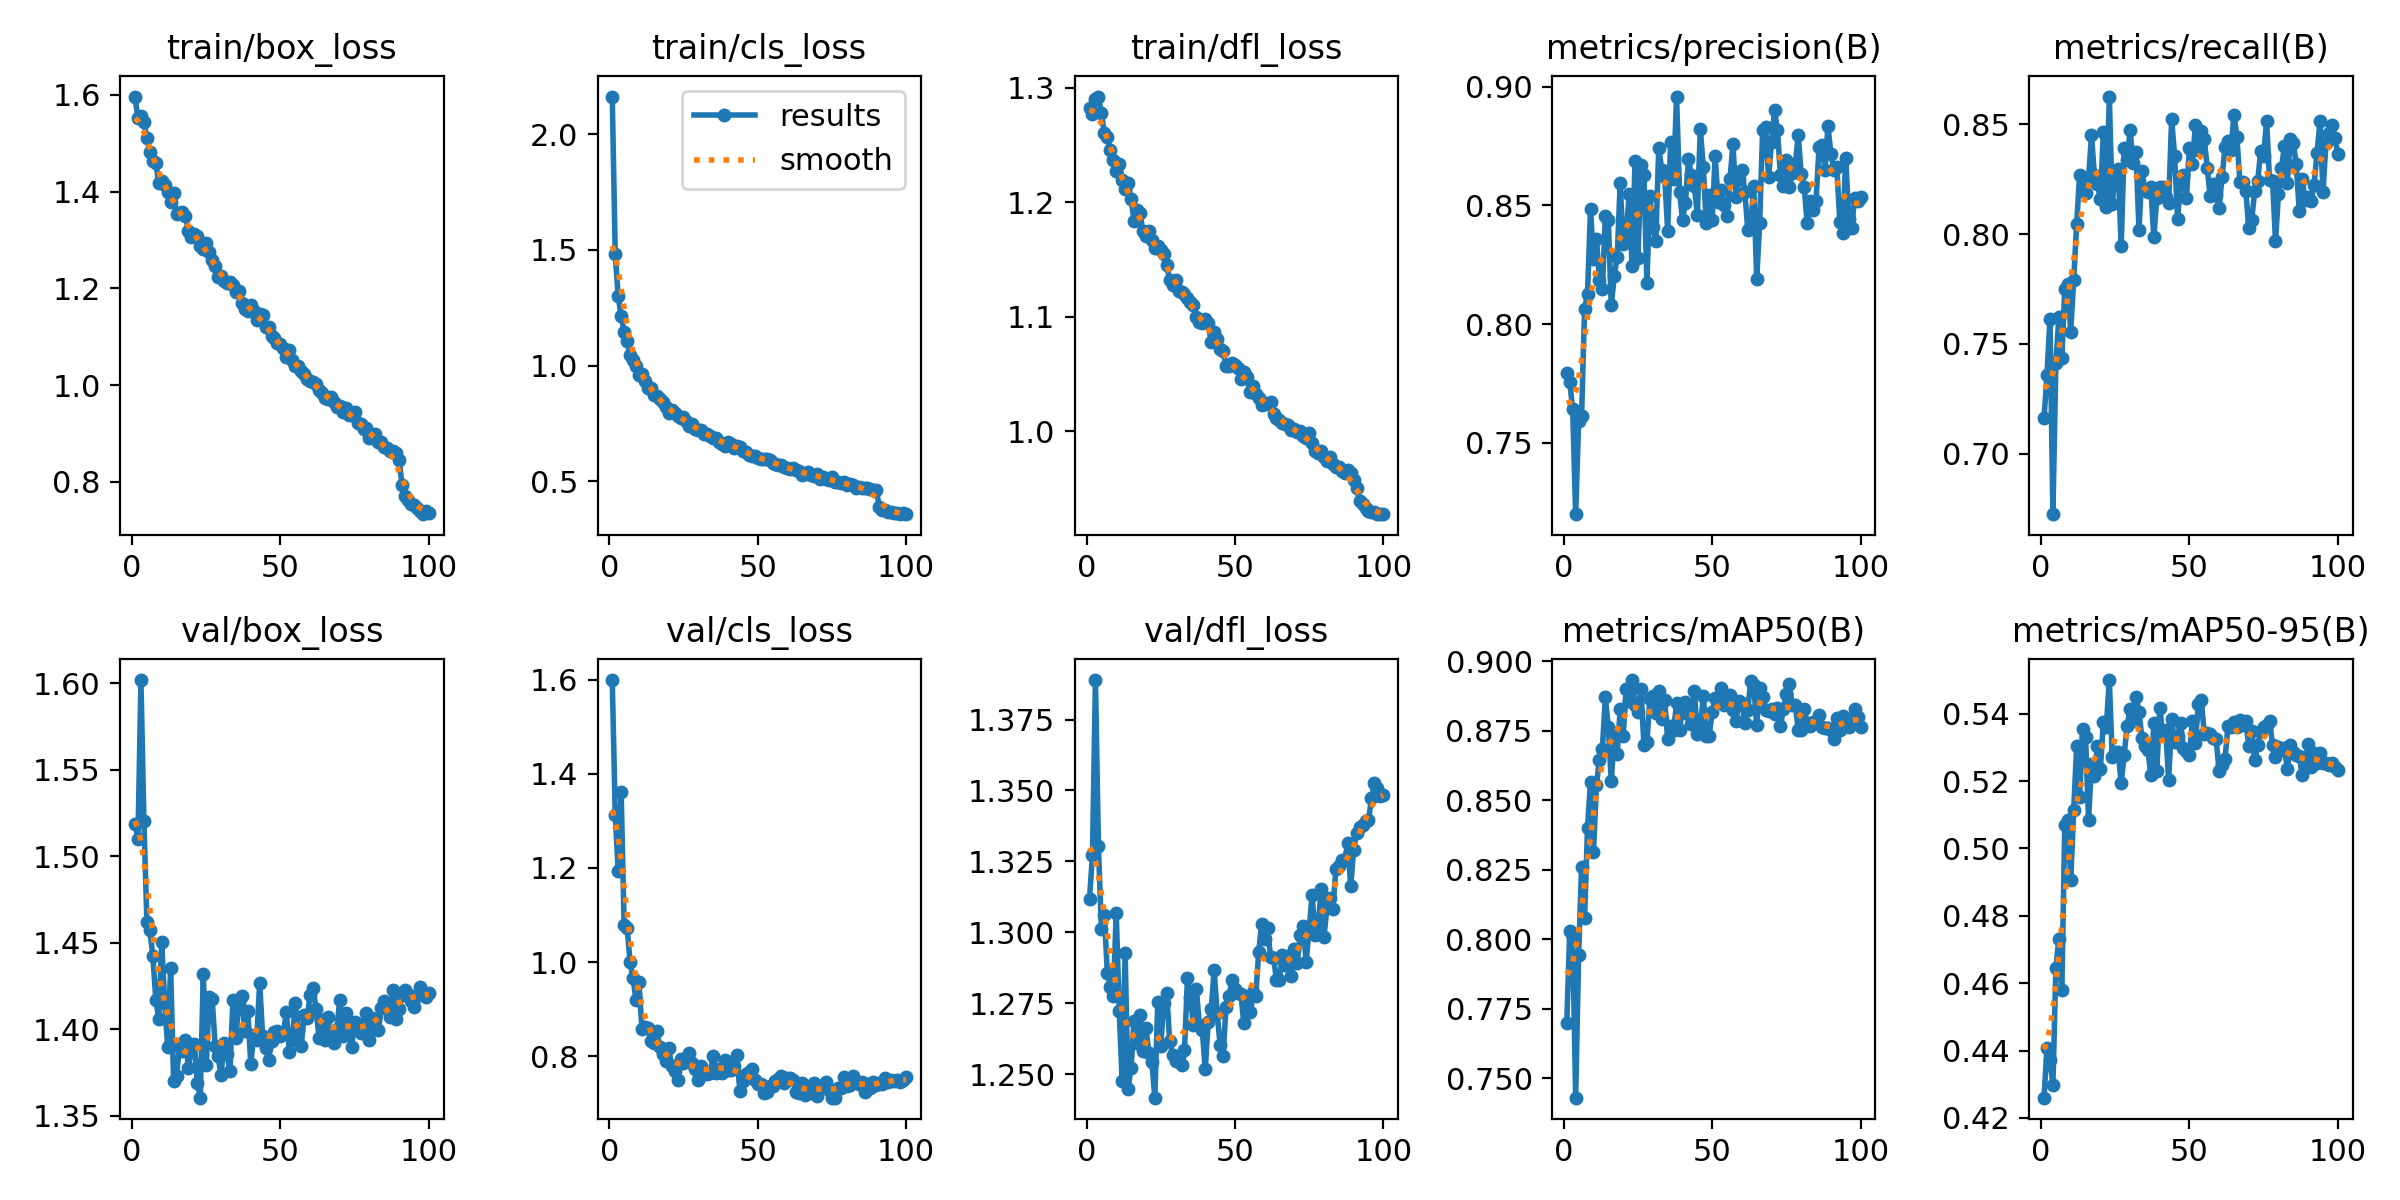
\includegraphics[width=0.8\textwidth]{figures/model_results/helmet_model_results.png}
    \caption{Training summary for the helmet compliance model.}
    \label{fig:helmet-model-results}
\end{figure}

The precision--recall (PR) curve in Figure~\ref{fig:pr-curve} characterizes the trade-off between precision and recall across confidence thresholds. This diagnostic is used to select operational thresholds appropriate for enforcement settings, where false positives must be controlled while maintaining adequate recall for safety-critical violations.
\begin{figure}[htbp]
    \centering
    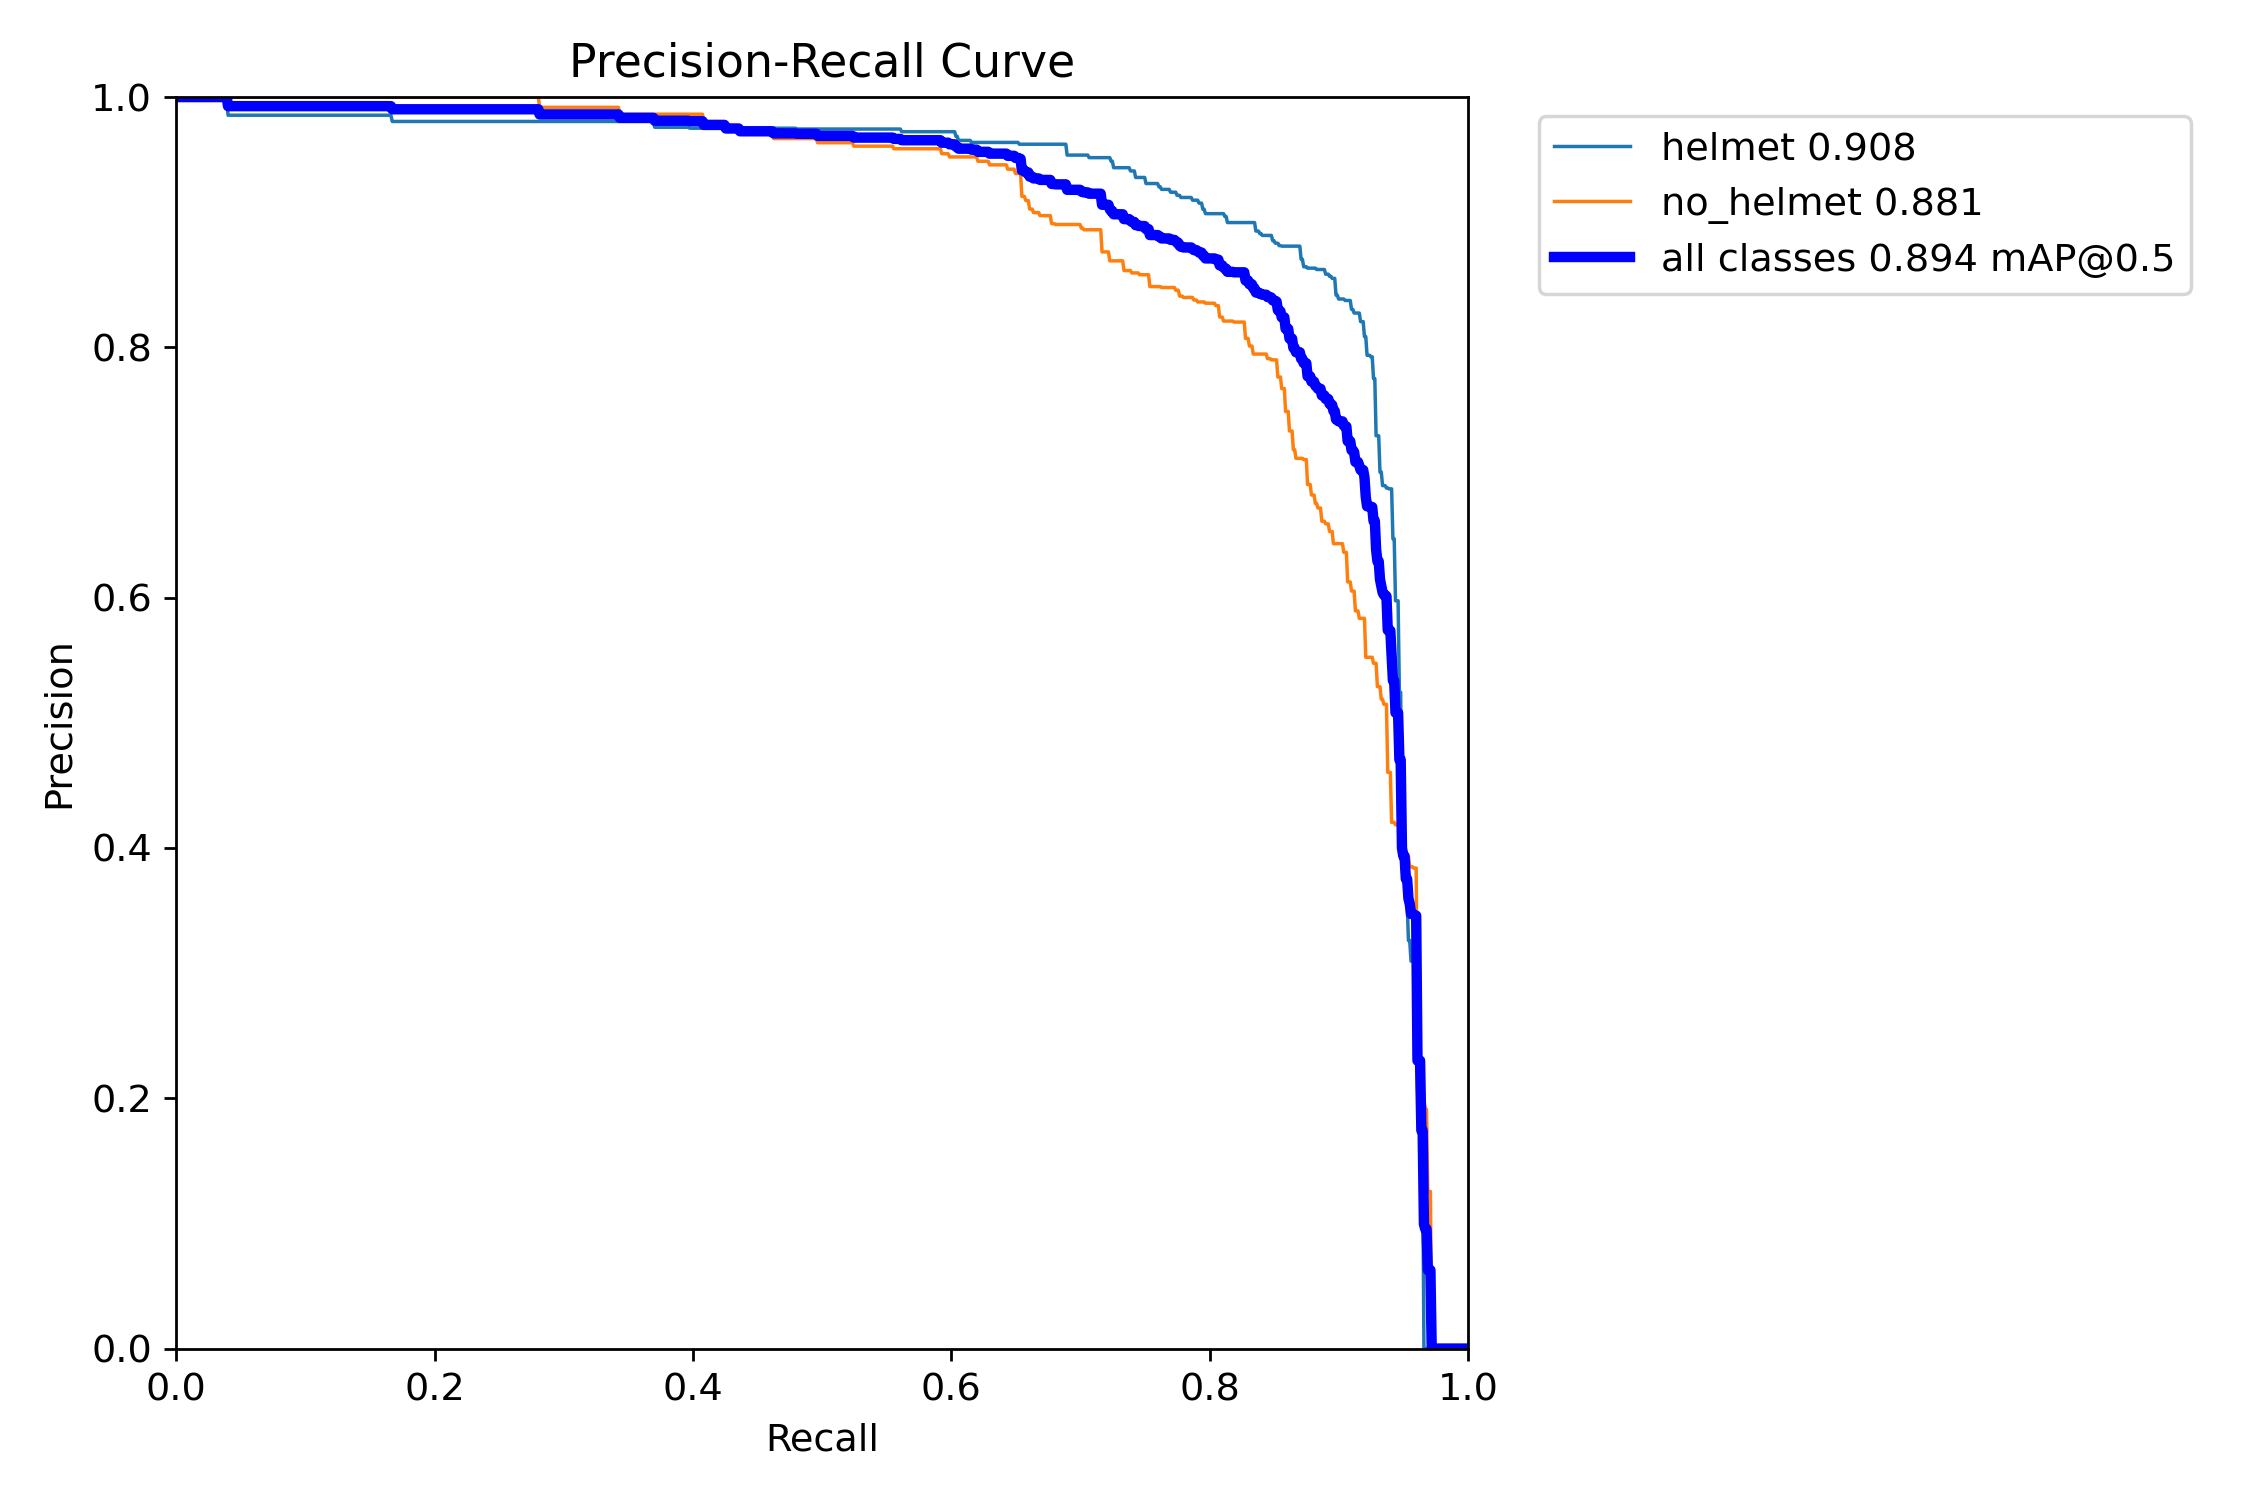
\includegraphics[width=0.8\textwidth]{figures/model_results/Helmet_BoxPR_curve.png}
    \caption{Precision--recall curve for the trained detection/classification pipeline (intermediate).}
    \label{fig:pr-curve}
\end{figure}

The confusion matrix in Figure~\ref{fig:confusion-matrix} presents class-wise error distribution and provides insight into systematic misclassifications (e.g., confusion between visually similar classes due to occlusion, motion blur, and small object scale). These observations directly inform dataset refinement and targeted augmentation strategies.
\begin{figure}[htbp]
    \centering
    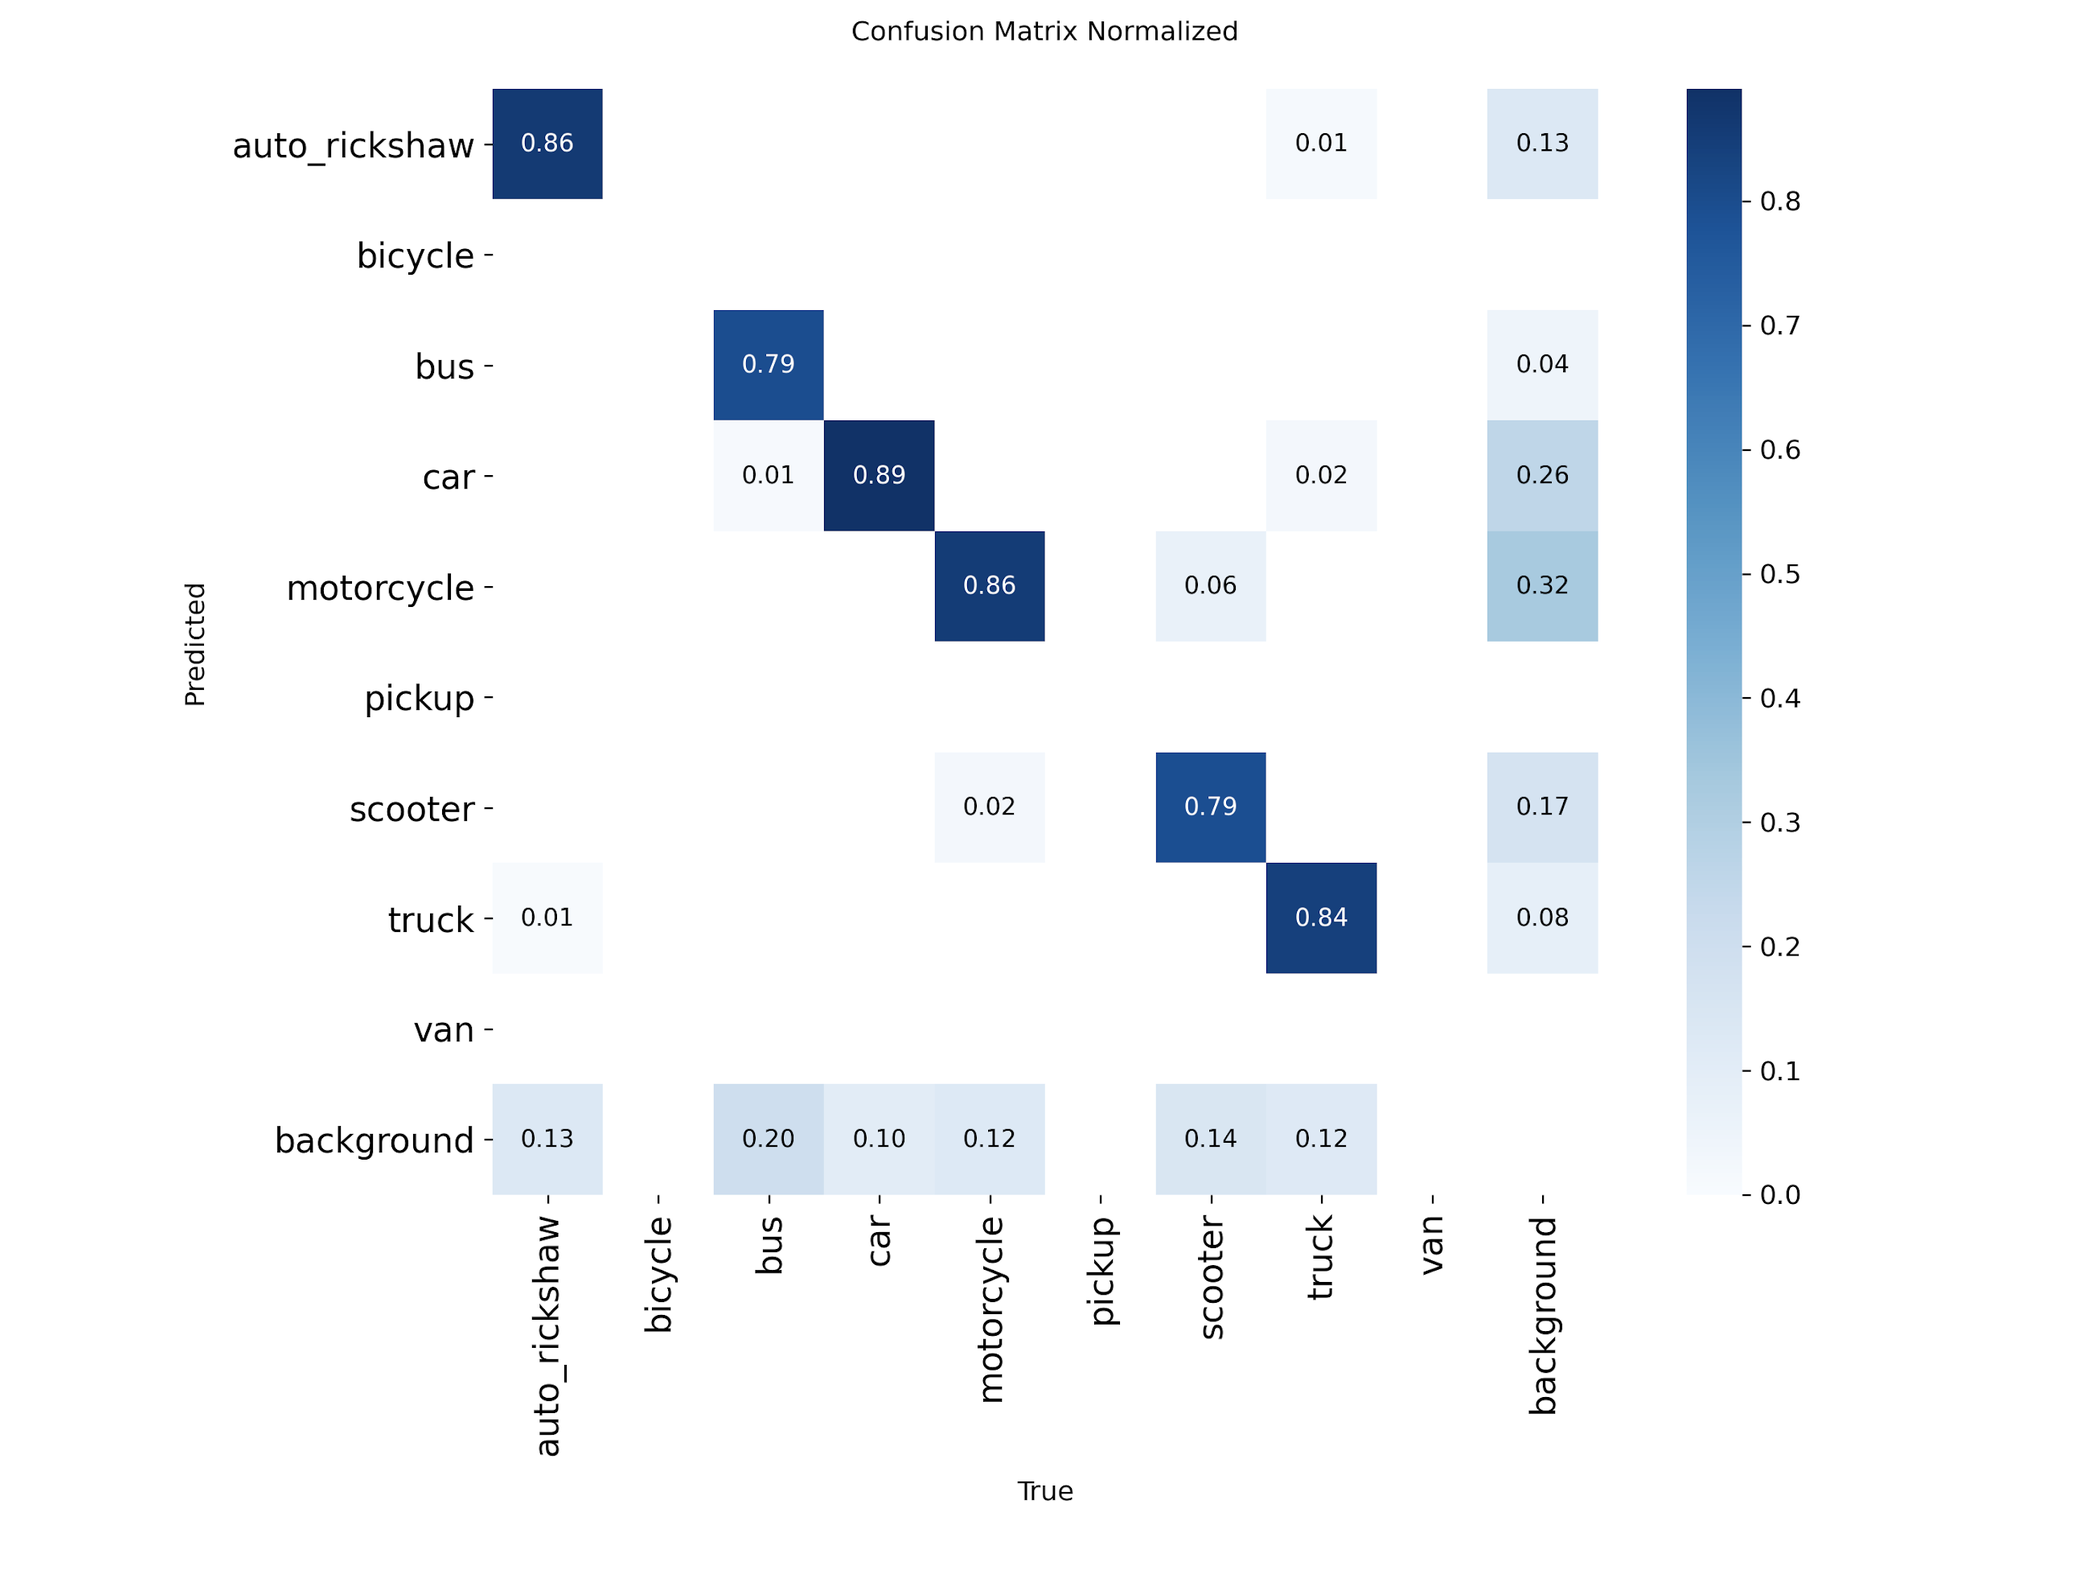
\includegraphics[width=0.8\textwidth]{figures/model_results/normalized_confusion_vehicle_detect.png}
    \caption{Normalized confusion matrix for the current vehicle detection model (intermediate).}
    \label{fig:confusion-matrix}
\end{figure}

\subsection{Preliminary System Interface Views}
\label{subsec:preliminary-system-interface}

Figure~\ref{fig:admin-view} demonstrates the Admin interface used to manage users, configure system parameters, and monitor operational status at a high level. This view supports governance and access management to ensure that only authorized personnel can approve enforcement actions or modify core system settings.
\begin{figure}[htbp]
    \centering
    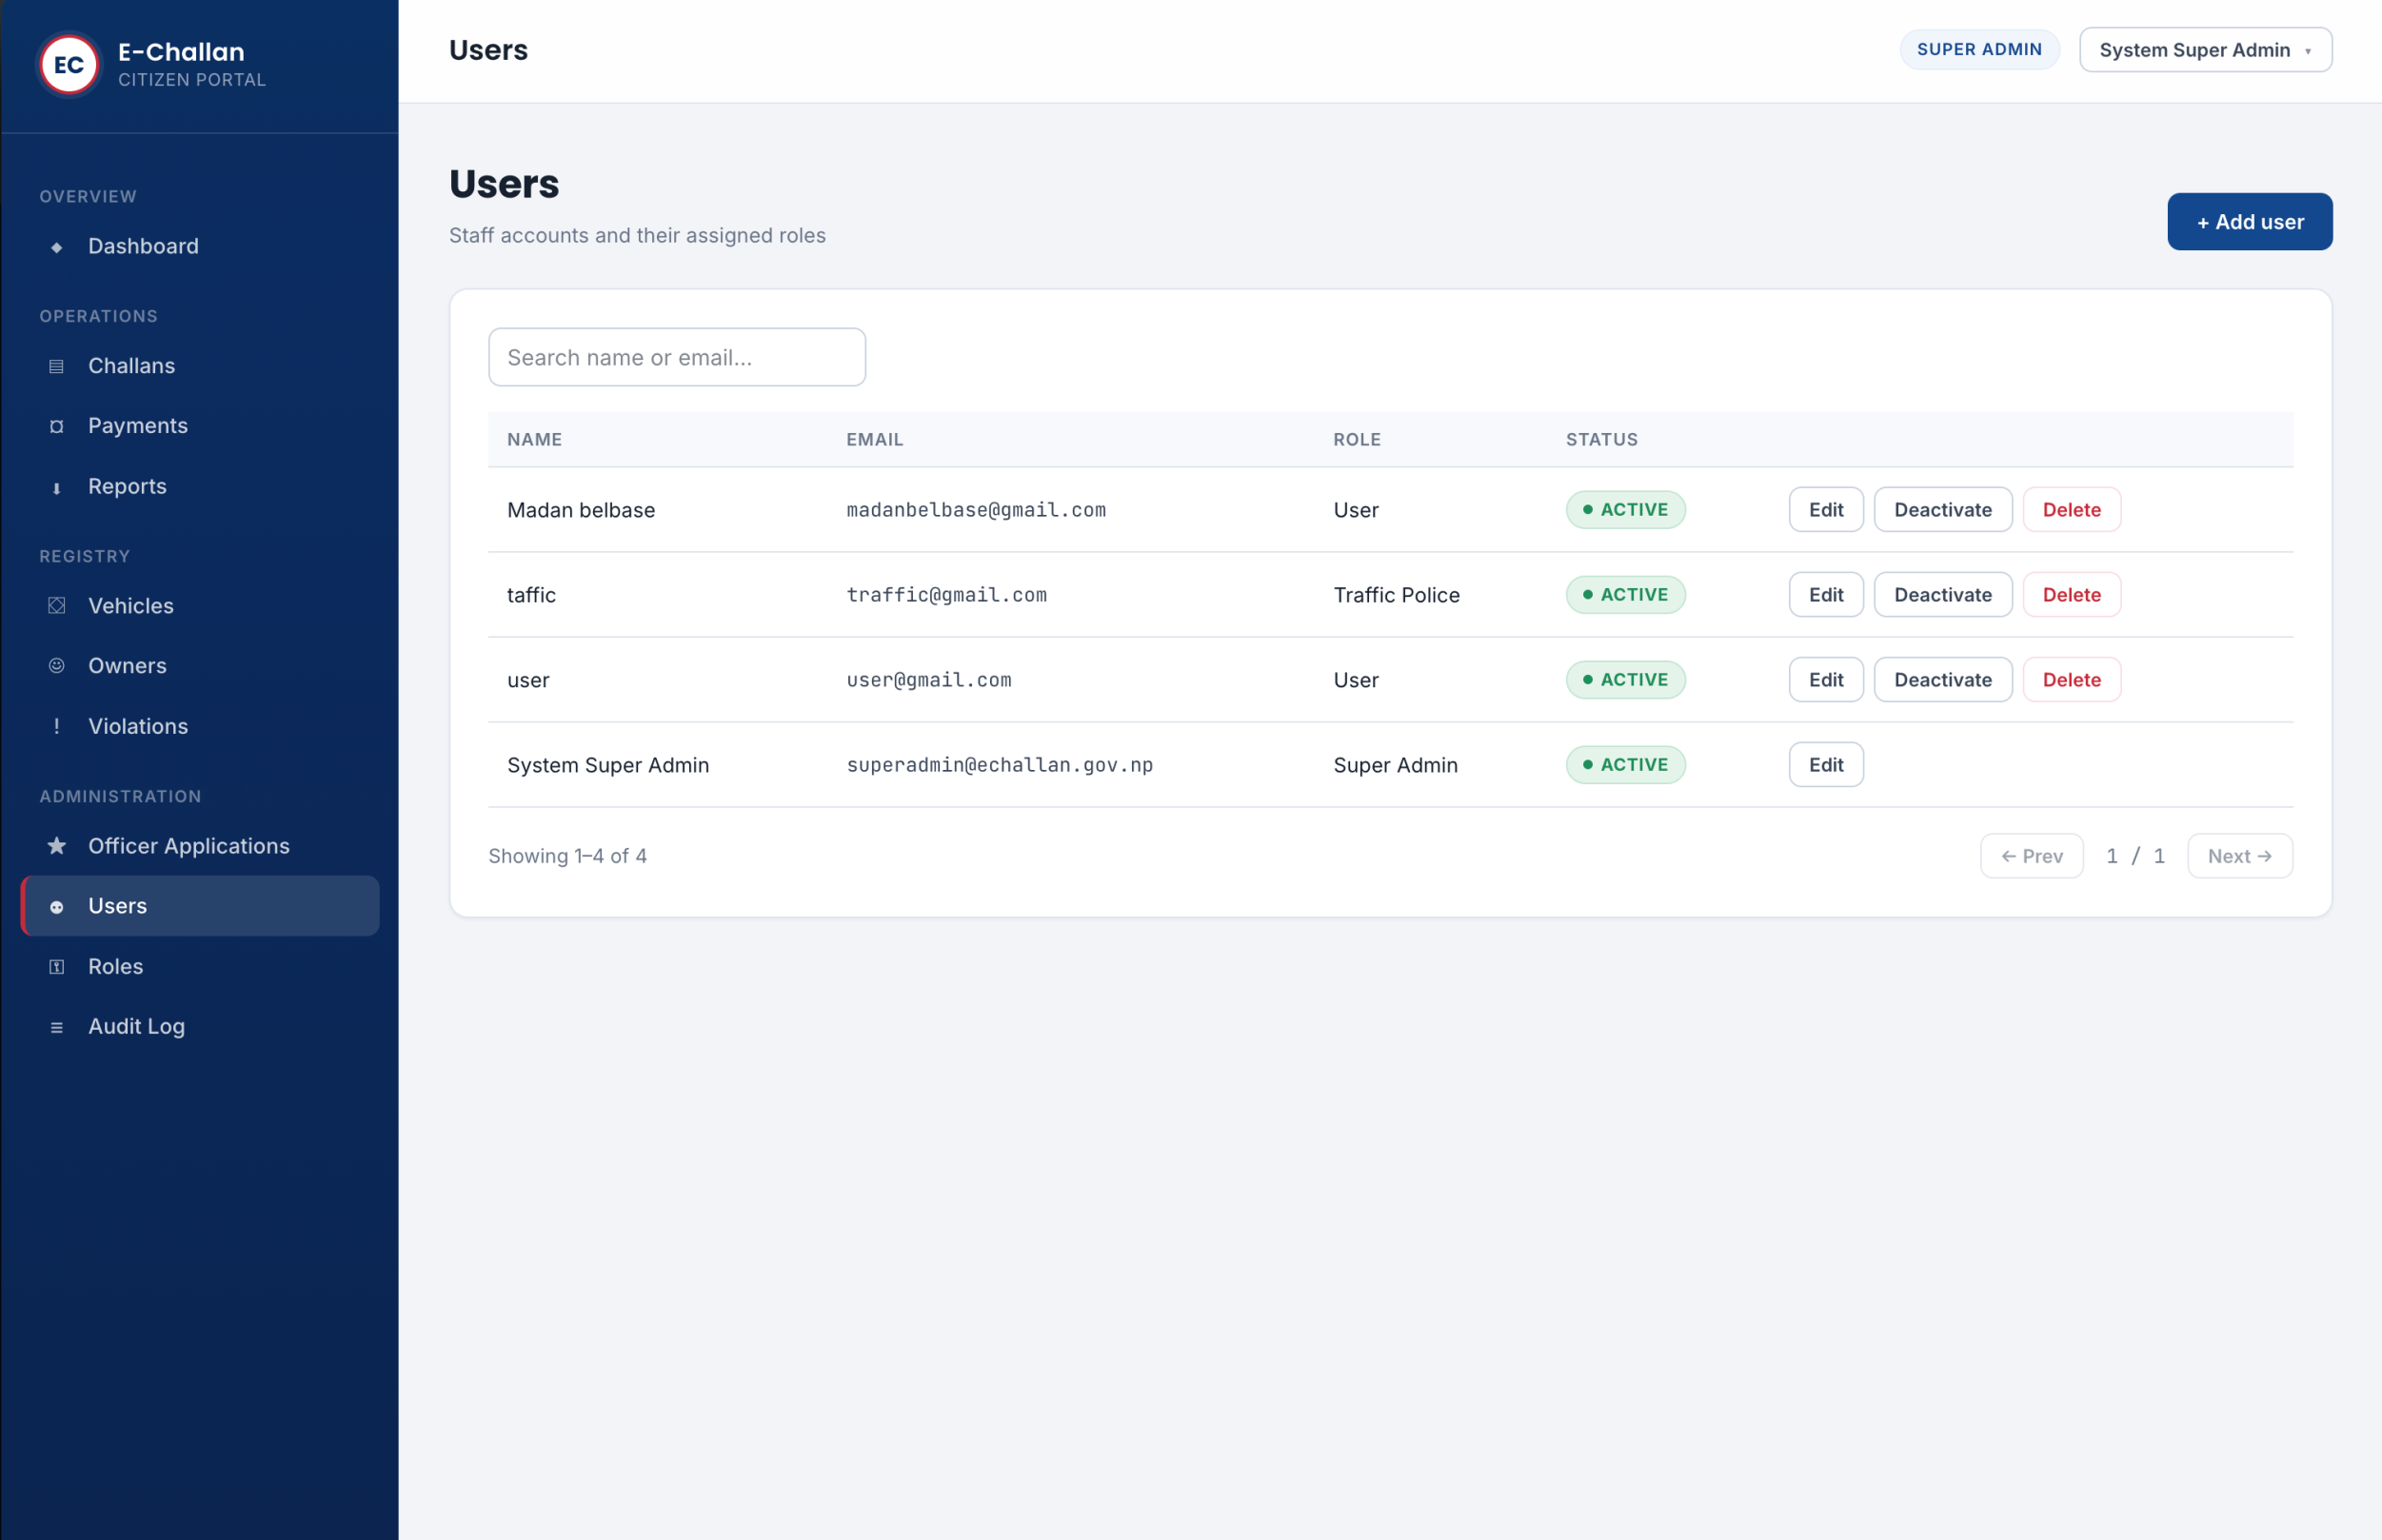
\includegraphics[width=0.8\textwidth]{figures/backend_frontend_figures/super_admin_manage_users.png}
    \caption{Role-based Admin view for user and system management.}
    \label{fig:admin-view}
\end{figure}

Figure~\ref{fig:traffic-officer-view} presents the Traffic Police interface designed for evidence verification, violation review, and challan approval. The layout prioritizes rapid decision-making by displaying essential metadata (time, location, violation type) alongside evidence media and verification actions.
\begin{figure}[htbp]
    \centering
    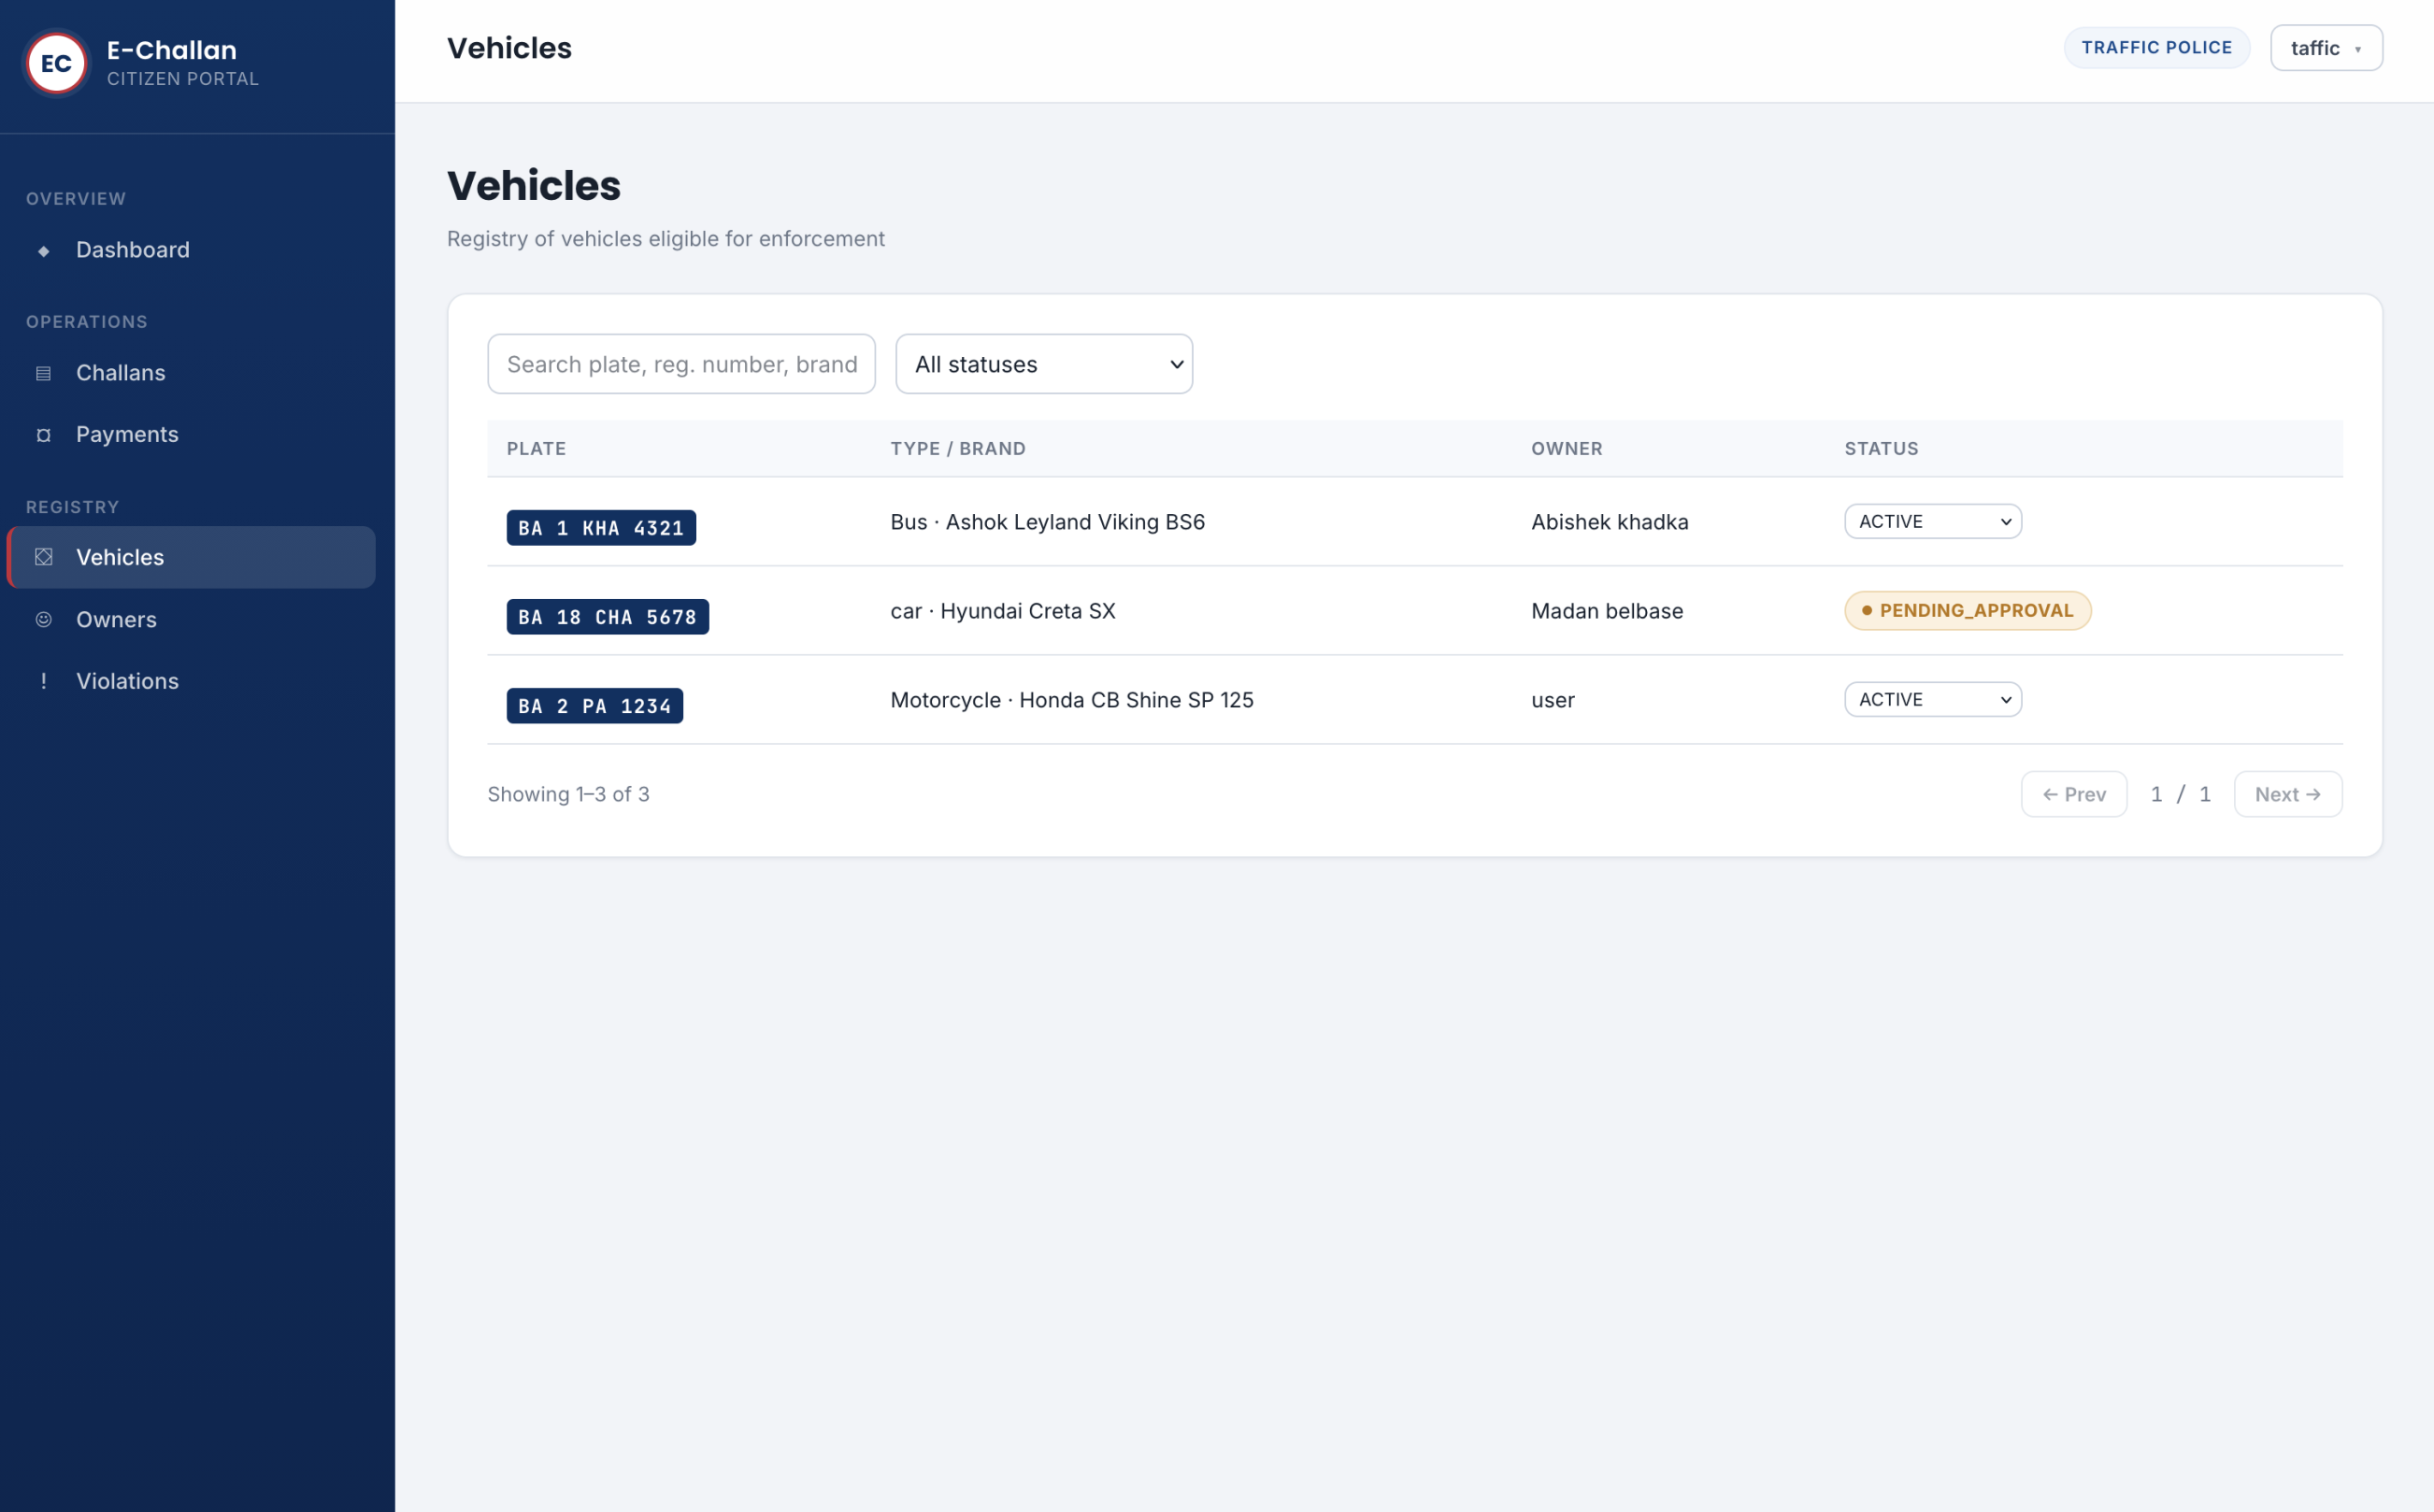
\includegraphics[width=0.8\textwidth]{figures/backend_frontend_figures/traffic_view.png}
    \caption{Traffic Police view for reviewing violations and validating e-challans.}
    \label{fig:traffic-officer-view}
\end{figure}

Figure~\ref{fig:user-view} shows the general user-facing dashboard concept, intended to provide transparent access to issued challans, violation history, and payment-related tracking. This interface supports accountability and reduces friction in fine settlement processes by centralizing challan details and evidence references.
\begin{figure}[htbp]
    \centering
    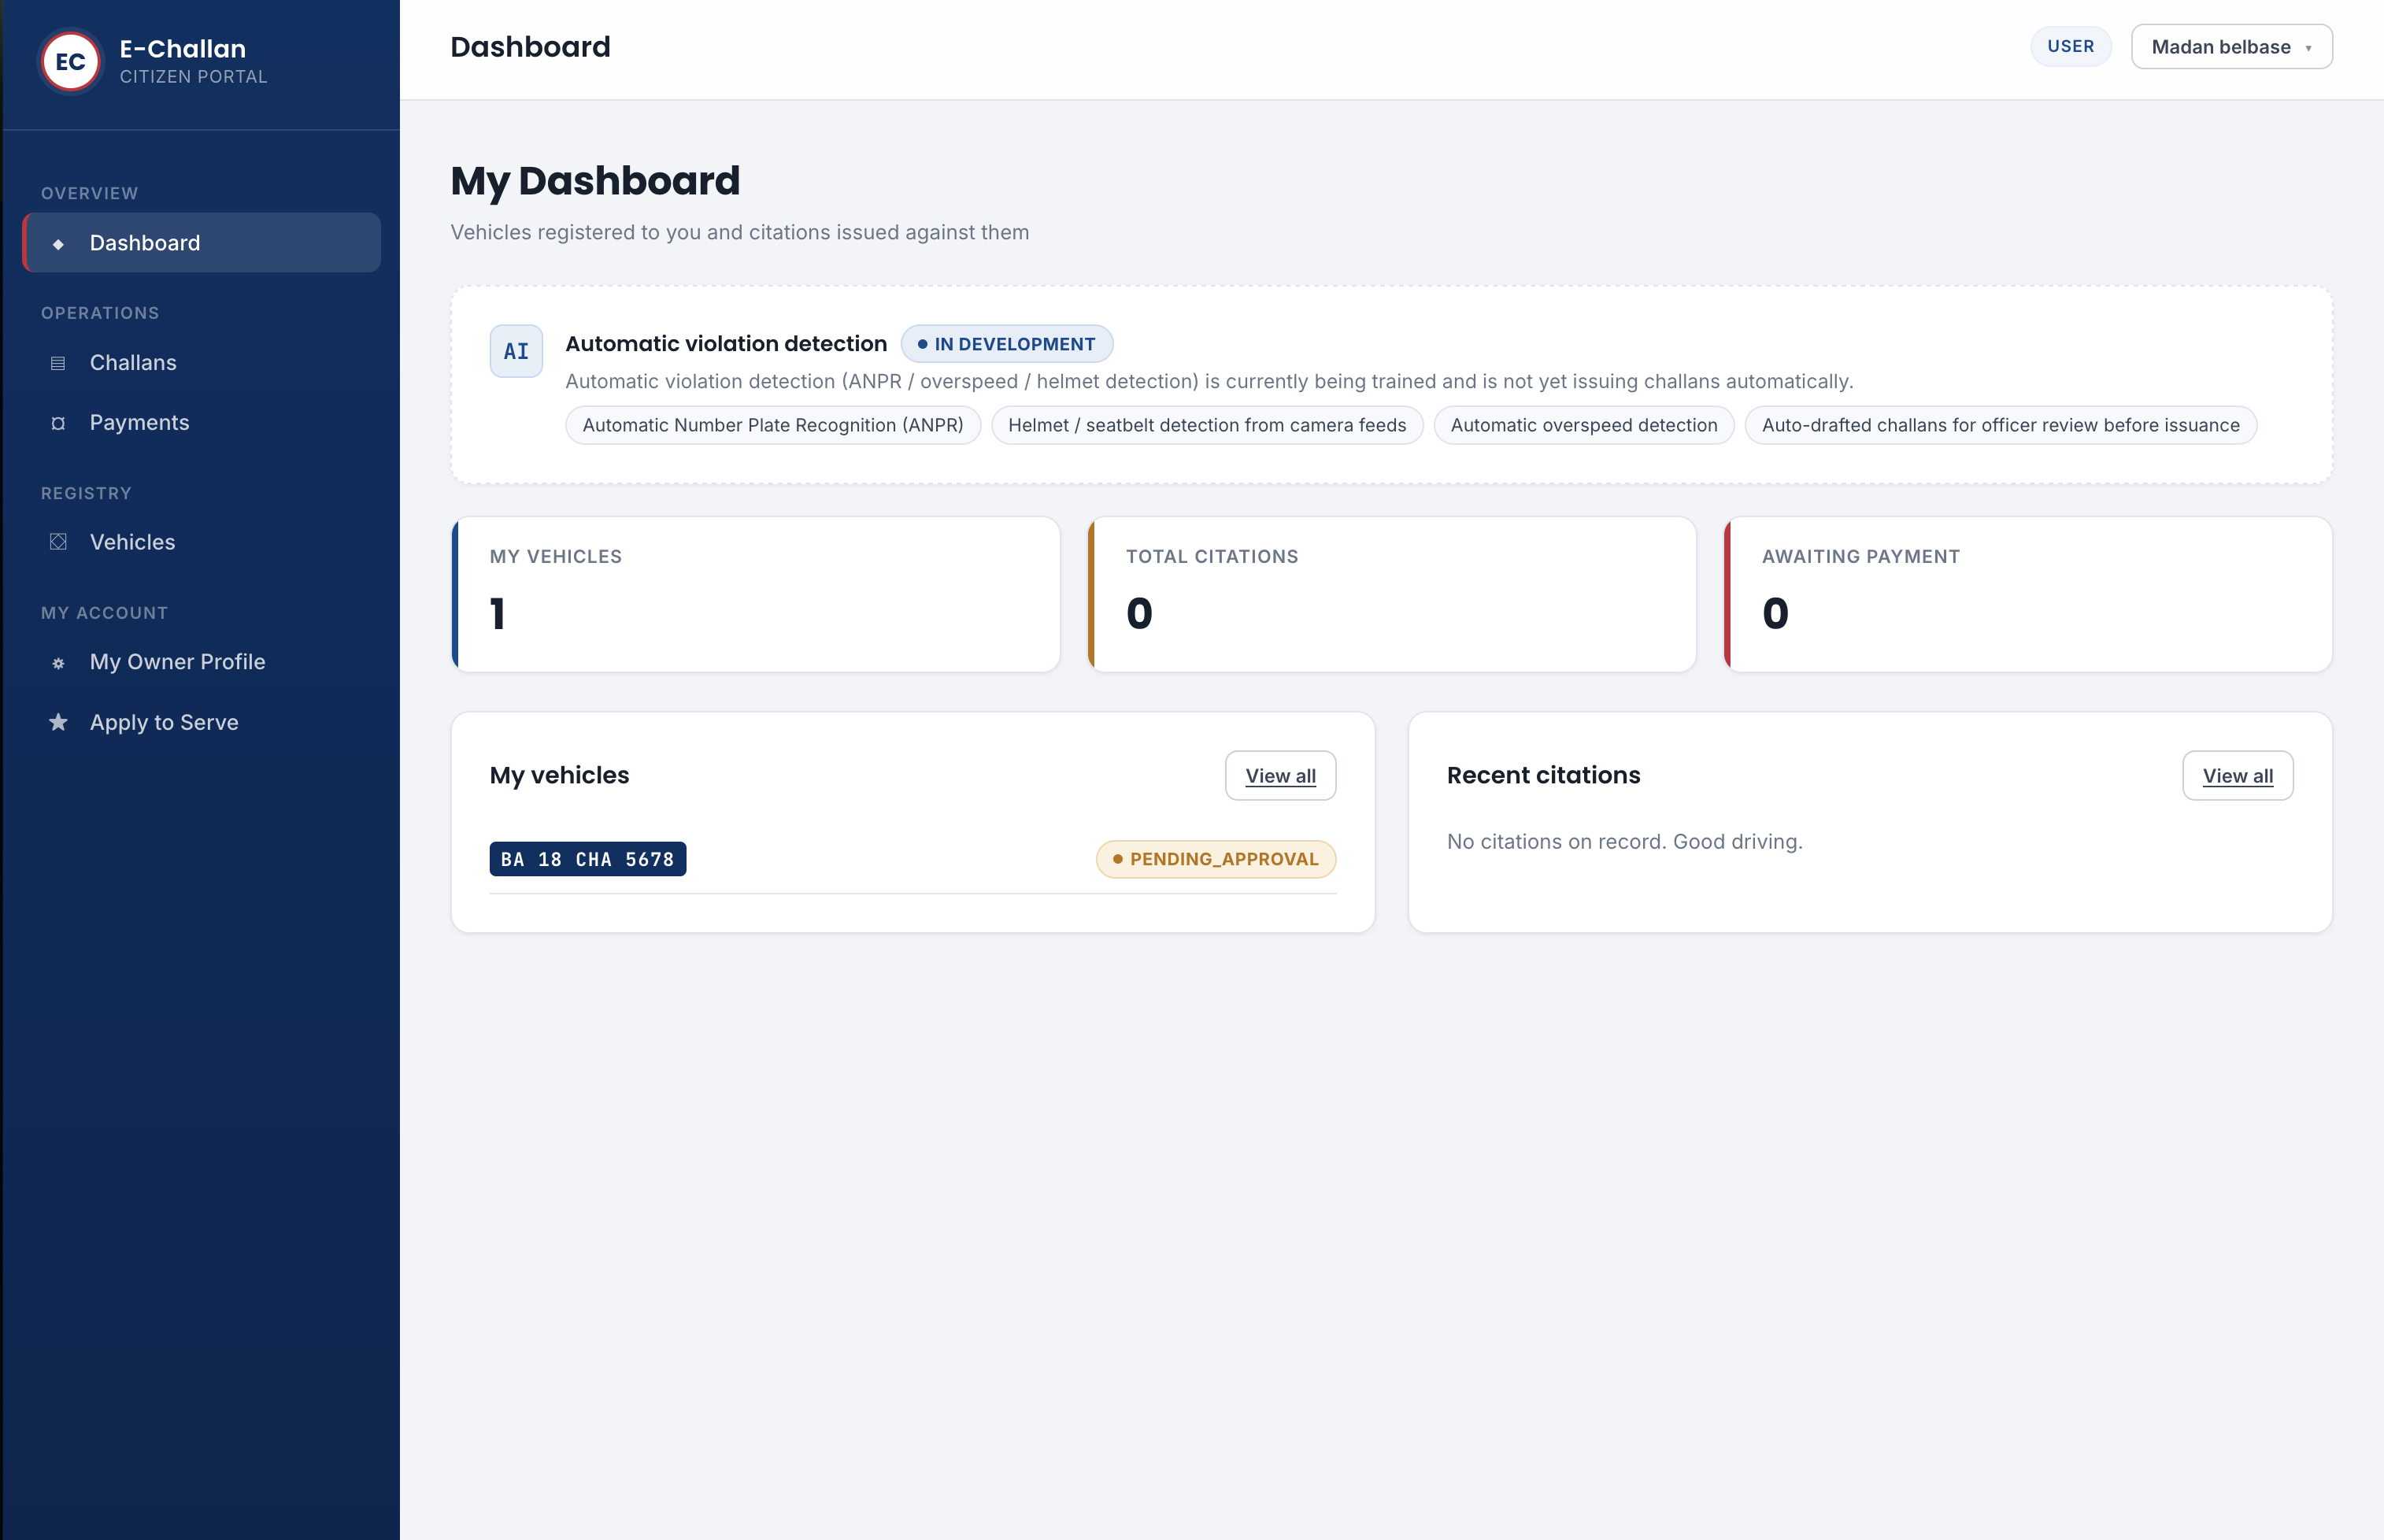
\includegraphics[width=0.8\textwidth]{figures/backend_frontend_figures/user_dashboard.png}
    \caption{General user view for challan history and fine tracking.}
    \label{fig:user-view}
\end{figure}

\section{Remaining Work}
\label{sec:remaining-work}

\subsection{System Integration}
\label{subsec:system-integration}
The final phase will prioritize end-to-end integration of the ML inference pipeline with the service layer and user interfaces. This includes connecting real-time inference outputs (detections, classifications, OCR strings, and confidence scores) to the FastAPI/Node.js backend, designing stable event payloads, implementing evidence storage workflows, and ensuring that the React dashboard receives real-time updates with consistent status transitions (e.g., \textit{Detected} $\rightarrow$ \textit{Pending Review} $\rightarrow$ \textit{Approved/Rejected} $\rightarrow$ \textit{Challan Issued}).

\subsection{Additional Model Training and Implementation}
\label{subsec:additional-models}
Two additional violation categories will be implemented to complete the multi-violation scope:
\begin{itemize}
    \item \textbf{Triple Riding Detection:} Extend the detection pipeline to associate multiple riders with each motorcycle and reliably estimate rider count under occlusions and varying camera angles.
    \item \textbf{Mobile Phone Usage Detection:} Train and deploy a specialized detector/classifier to identify handheld mobile usage by riders, accounting for small object size, motion blur, and partial occlusion.
\end{itemize}

\subsection{Mobile Application Development}
\label{subsec:mobile-app}
A lightweight mobile application will be developed to support on-the-go monitoring for authorized traffic personnel and fine tracking for vehicle owners. The planned application will integrate with the same backend APIs to provide authenticated access, notification support, and a streamlined interface for viewing violations, evidence media, and challan payment status.
\end{enumerate}
\newpage

\section{Performance Analysis and Validation}
\input{chapters/performance-analysis-validation}
\newpage

\section{Ethical Concerns}
\input{chapters/ethical-concerns}
\newpage

\section{Results and Discussion}

\label{ch:results-discussion}

This chapter summarizes the progress achieved up to the mid-term defense. Since the system is under active development, the results reported here are preliminary and are intended to validate feasibility, guide further model tuning, and identify risks before final deployment.

\section{Implementation Status (Mid-Term)}
\label{sec:impl-status}

At the time of mid-term review, the project has been implemented as a modular pipeline with clearly separated components:
\begin{itemize}
    \item Video ingestion and frame extraction from recorded CCTV samples (with RTSP support planned for final integration).
    \item Object detection for motorcycle and rider localization using YOLOv8.
    \item Helmet compliance detection based on cropped rider/head regions.
    \item Rider counting logic for triple-riding violation detection.
    \item Number plate detection and OCR integration in a prototype stage.
    \item A preliminary backend API and database schema design for storing violations and evidence.
\end{itemize}

\section{Dataset Preparation Summary}
\label{sec:dataset-summary}

Public datasets listed in Chapter~3 were inspected and standardized into a YOLO-compatible directory structure. During preprocessing, corrupted images were removed, class labels were normalized across sources, and image resolutions were unified to match the selected training configuration. The dataset split followed the planned ratios (training/validation/testing), and augmentation strategies (flip, brightness/contrast, and small rotations) were applied during training to improve generalization.

\section{Preliminary Model Training Results}
\label{sec:prelim-training}

\subsection{Motorcycle and Rider Detection}
A YOLOv8 detector was trained/fine-tuned to identify motorcycles and rider/person instances from traffic scenes. Early experiments indicate stable detections in daylight and moderate traffic density. Failure cases are mostly associated with heavy occlusion, distant riders, and low-resolution frames.

\subsection{Helmet Compliance Detection}
Helmet detection was evaluated on cropped rider regions. The model produces reliable predictions when the rider's head region is clearly visible. False negatives were observed in cases of motion blur and when helmets are partially occluded by the rider posture or camera angle.

\subsection{Triple-Riding Detection}
Triple riding is currently determined by associating detected rider instances with a detected motorcycle and counting riders per vehicle. Preliminary tests show that rider counting is sensitive to:
\begin{itemize}
    \item missed rider detections under occlusion,
    \item double-counting in crowded backgrounds,
    \item perspective changes when motorcycles move across the field of view.
\end{itemize}
In the final phase, a tracking module (e.g., ByteTrack/DeepSORT) will be integrated to stabilize counts across consecutive frames and reduce duplicate violation triggers.

\section{Prototype ANPR and OCR Observations}
\label{sec:anpr-ocr}

A two-step approach is being followed: (i) number plate localization using an object detector and (ii) character extraction using OCR (EasyOCR/PaddleOCR). In preliminary experiments, plate text extraction works best when the plate occupies a sufficient number of pixels and is near-frontal. OCR confidence drops significantly due to motion blur, glare, and non-standard fonts.

\section{System-Level Output (Evidence Generation)}
\label{sec:evidence}

For each detected violation event, the prototype pipeline produces:
\begin{itemize}
    \item a cropped evidence image showing the motorcycle/rider,
    \item metadata (timestamp and camera identifier),
    \item the predicted violation type (no-helmet and/or triple riding),
    \item a provisional number plate string (when OCR succeeds).
\end{itemize}
The mid-term objective has been to confirm that these artifacts can be generated automatically and stored for subsequent review in the dashboard.

\section{Discussion}
\label{sec:discussion}

\subsection{Feasibility and Key Findings}
The preliminary results support the feasibility of real-time two-wheeler violation detection using a YOLOv8-based pipeline. In controlled samples, the detector provides consistent localization of motorcycles and riders, enabling downstream rule checks for helmet compliance and rider count.

\subsection{Primary Challenges}
The most important challenges identified during mid-term development are:
\begin{itemize}
    \item \textbf{Occlusion and crowding:} overlapping objects reduce detection and counting reliability.
    \item \textbf{Low-quality footage:} blur and compression artifacts degrade helmet and OCR performance.
    \item \textbf{Camera geometry:} distant viewpoints reduce the effective resolution of head and plate regions.
    \item \textbf{Duplicate events:} without tracking, the same motorcycle may be flagged repeatedly across frames.
\end{itemize}

\subsection{Planned Improvements for Final Defense}
To address the above limitations, the next development phase will focus on:
\begin{itemize}
    \item integrating multi-object tracking to create stable vehicle identities across frames,
    \item improving helmet detection robustness with additional training samples and augmentation,
    \item strengthening ANPR by tuning plate detection and applying OCR post-processing (regex-based cleaning and confidence thresholds),
    \item implementing event de-duplication and temporal rules (violation confirmed only after consistent detection across $N$ consecutive frames),
    \item completing backend integration (FastAPI endpoints, database persistence, and dashboard views).
\end{itemize}

\section{Summary}
\label{sec:results-summary}

At mid-term, the core detection pipeline has been prototyped and validated on sample traffic footage. The results highlight that accurate detection is achievable under favorable conditions, while robustness under occlusion and low-quality video remains the key area for improvement. The next phase will prioritize tracking, ANPR reliability, and end-to-end integration to support automated evidence logging and e-challan generation.

\newpage

\section{Project Task and Time schedule}
\begin{table}[H]
\centering
\begin{tabularx}{\textwidth}{|l|X|l|}
\hline
\textbf{Phase} & \textbf{Activities} & \textbf{Status} \\
\hline
Literature Study & Review YOLO-based detection, helmet detection approaches, OCR for number plates & Completed \\
\hline
Dataset \/ Input Setup & Collect sample videos, define target classes, set preprocessing pipeline & In progress \\
\hline
Detection Prototype & Implement YOLOv8 inference on frames, visualize detections, tune thresholds & Completed \\
\hline
Violation Logic & Define helmet rule, temporal smoothing, reduce false positives & In progress \\
\hline
Number Plate OCR & Plate ROI extraction, OCR integration, preprocessing experiments &Completed \\
\hline
E-Challan Output & Design record format, evidence saving, duplicate prevention per track & Completed \\
\hline
Evaluation & Metrics, FPS benchmarking, error case analysis & Planned \\
\hline
Report Writing & Mid-term report drafting and formatting & In progress \\
\hline
\end{tabularx}
\caption{Project task schedule and current status}
\end{table}

\newpage

\section{Conclusion}
This mid-term report outlined the motivation, objectives, and methodology for developing an automated two-wheeler violation detection and e-challan generation system using YOLOv8 and OpenCV. The work completed so far includes setting up the development environment, reviewing relevant literature, and developing an initial detection pipeline for riders and helmets. The next phase will focus on improving violation decision logic, integrating robust number plate OCR, generating structured e-challan outputs with evidence, and performing systematic evaluation under different video conditions.

\newpage

\section*{References}
\addcontentsline{toc}{section}{References}
\raggedright

\printbibliography[heading=none]
\newpage
\section{Abbreviations}

 % %\input{chapters/abbreviation}
\newpage

\section{Appendix}
 % %\input{chapters/appendix}
\newpage

\end{document}